\chapter{Clustering}
\label{chapter:ivf}

\abstract{
We have seen index structures that manifest as trees, hash tables, and graphs.
In this chapter, we will introduce a fourth way of organizing data points: clusters.
It is perhaps the most natural and the simplest of the four methods,
but also the least theoretically-justified. We will see why that is as we describe
the details of clustering-based algorithms to top-$k$ retrieval.
}

\section{Algorithm}
\label{section:ivf:retrieval}

As usual, we begin by indexing a collection of $m$ data points $\mathcal{X} \subset \mathbb{R}^d$.
Except in this paradigm, that involves invoking a \textbf{clustering} function,
$\zeta: \mathbb{R}^d \rightarrow [C]$,
that is appropriate for the distance function $\delta(\cdot, \cdot)$,
to map every data point to one of $C$ clusters, where $C$ is an arbitrary parameter.
A typical choice for $\zeta$ is the KMeans algorithm
with $C = \mathcal{O}(\sqrt{m})$.
We then organize $\mathcal{X}$ into a \emph{table} whose row $i$ records the subset
of points that are mapped to the $i$-th cluster: $\zeta^{-1}(i) \triangleq \{ u \;|\; u \in \mathcal{X}, \; \zeta(u) = i \}$.

Accompanying the index is a \textbf{routing} function $\tau: \mathbb{R}^d \rightarrow [C]^\ell$.
It takes an arbitrary point $q$ as input and returns $\ell$ clusters that are more likely to contain
the nearest neighbor of $q$ with respect to $\delta$. In a typical instance of this framework
$\tau(\cdot)$ is defined as follows:
\begin{equation}
    \label{equation:ivf:centroid-based-routing}
    \tau(q) = \argmin^{(\ell)}_{i \in [C]} \delta \Bigg(q,\; \underbrace{\frac{1}{\lvert \zeta^{-1}(i) \rvert} \sum_{u \in \zeta^{-1}(i)} u}_{\mu_i} \Bigg),
\end{equation}
where $\mu_i$ is the \emph{centroid} of the $i$-th cluster.
In other words, $\tau(\cdot)$ simply solves the top-$\ell$ retrieval problem
over the collection of centroids!
We will assume that $\tau$ is defined as above in the remainder of this section.

When processing a query $q$, we take a two-step approach.
We first obtain the list of clusters returned by $\tau(q)$, then solve the top-$k$
retrieval problem over the union of the identified clusters.
Figure~\ref{figure:ivf:framework} visualizes this procedure.

Notice that, the search for top-$\ell$ clusters by using
Equation~(\ref{equation:ivf:centroid-based-routing})
and the secondary search over the clusters identified by $\tau$ are themselves instances of the approximate
top-$k$ retrieval problem. The parameter $C$ determines the amount of effort that must be spent
in each of the two phases of search: When $C=1$, the cluster retrieval problem is solved trivially,
whereas as $C \rightarrow \infty$, cluster retrieval becomes equivalent to top-$k$ retrieval over the
entire collection.
Interestingly, these operations can be delegated to a
subroutine that itself uses a tree-, hash-, graph-, or even a clustering-based solution.
That is, a clustering-based approach can be easily paired with any of the previously discussed methods!

This simple protocol---with some variant of KMeans as $\zeta$ and $\tau$ as in Equation~(\ref{equation:ivf:centroid-based-routing})---works well in
practice~\citep{auvolat2015clustering,pq,bruch2023bridging,invertedMultiIndex,chierichetti2007clusterPruning}. We present the results of our own experiments on various real-world datasets in
Figure~\ref{figure:ivf:clustering-performance}.
This method owes its success to the empirical phenomenon that real-world data points
tend to follow a multi-modal distribution,
naturally forming clusters around each mode. By identifying these clusters
and grouping data points together, we reduce the search space at the expense of retrieval
quality.

\begin{figure}[t]
    \centering
    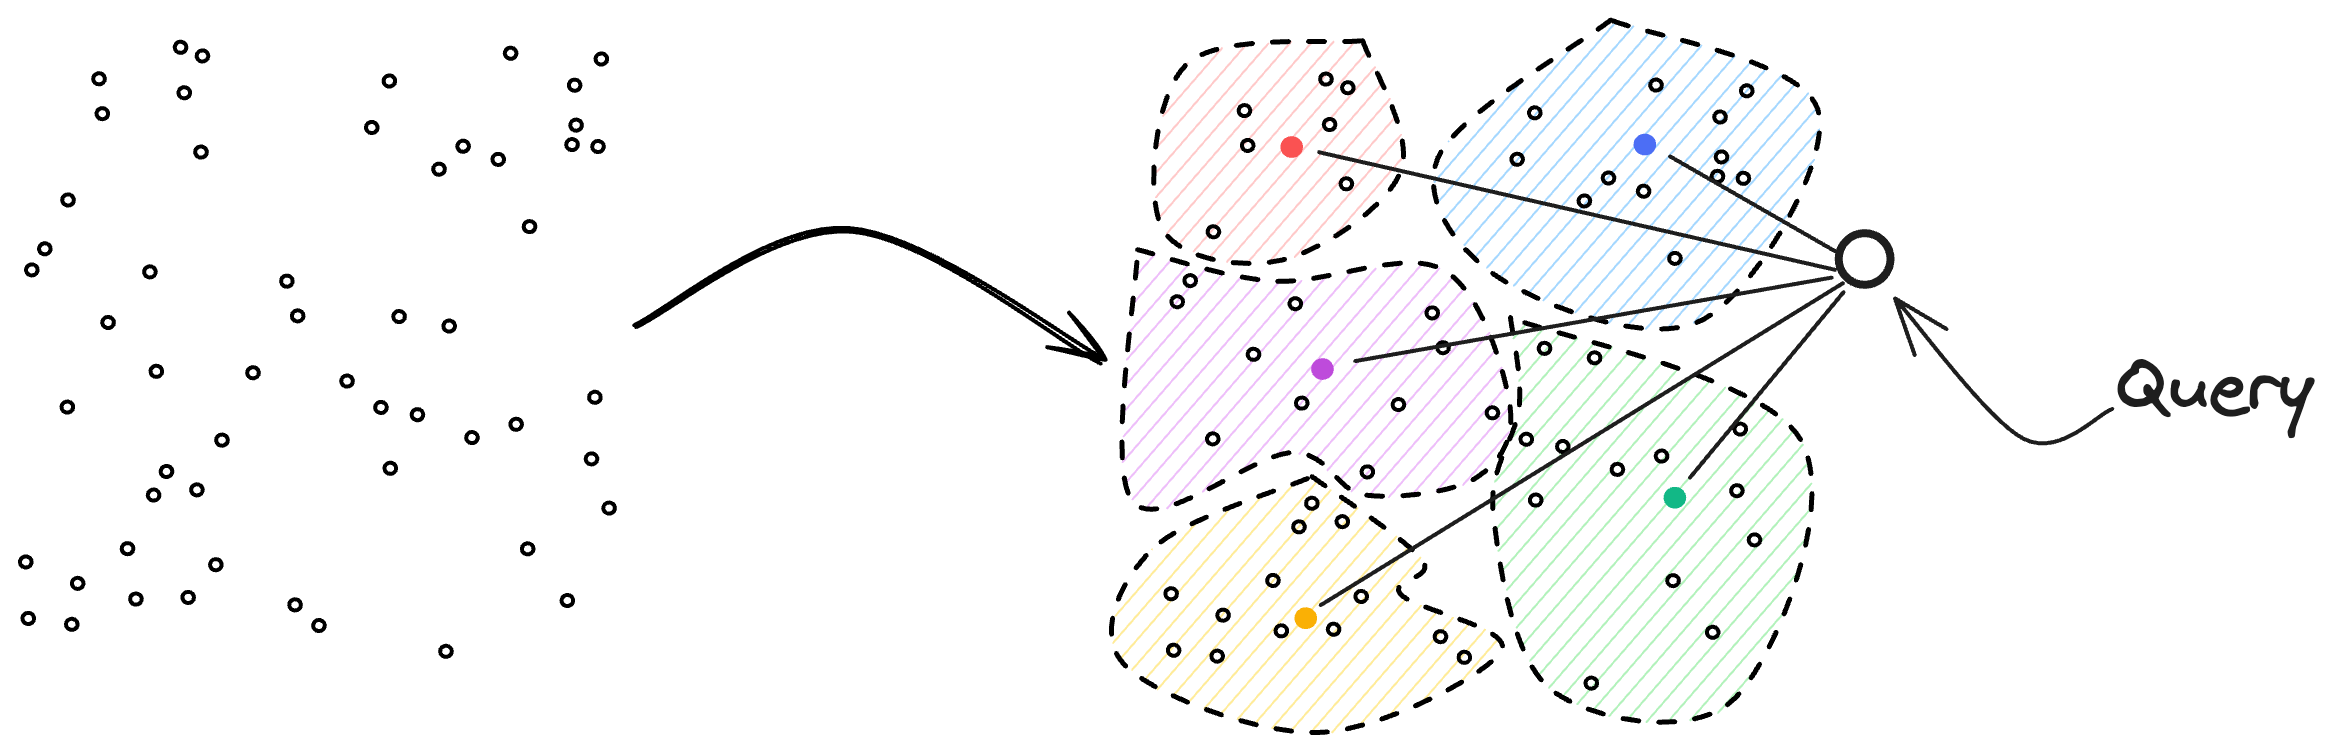
\includegraphics[width=0.8\linewidth]{figures/clustering-framework.png}
    \caption{Illustration of the clustering-based retrieval method. The collection of points
    (left) is first partitioned into clusters (regions enclosed by dashed boundary on the right).
    When processing a query $q$
    using Equation~(\ref{equation:ivf:centroid-based-routing}), we compute $\delta(q, \cdot)$ for
    the centroid (solid circles) of every cluster and conduct our search over the $\ell$ ``closest'' clusters.}
    \label{figure:ivf:framework}
\end{figure}

\begin{figure}[t]
    \centering
    \subfloat[\textsc{MIPS}]{
        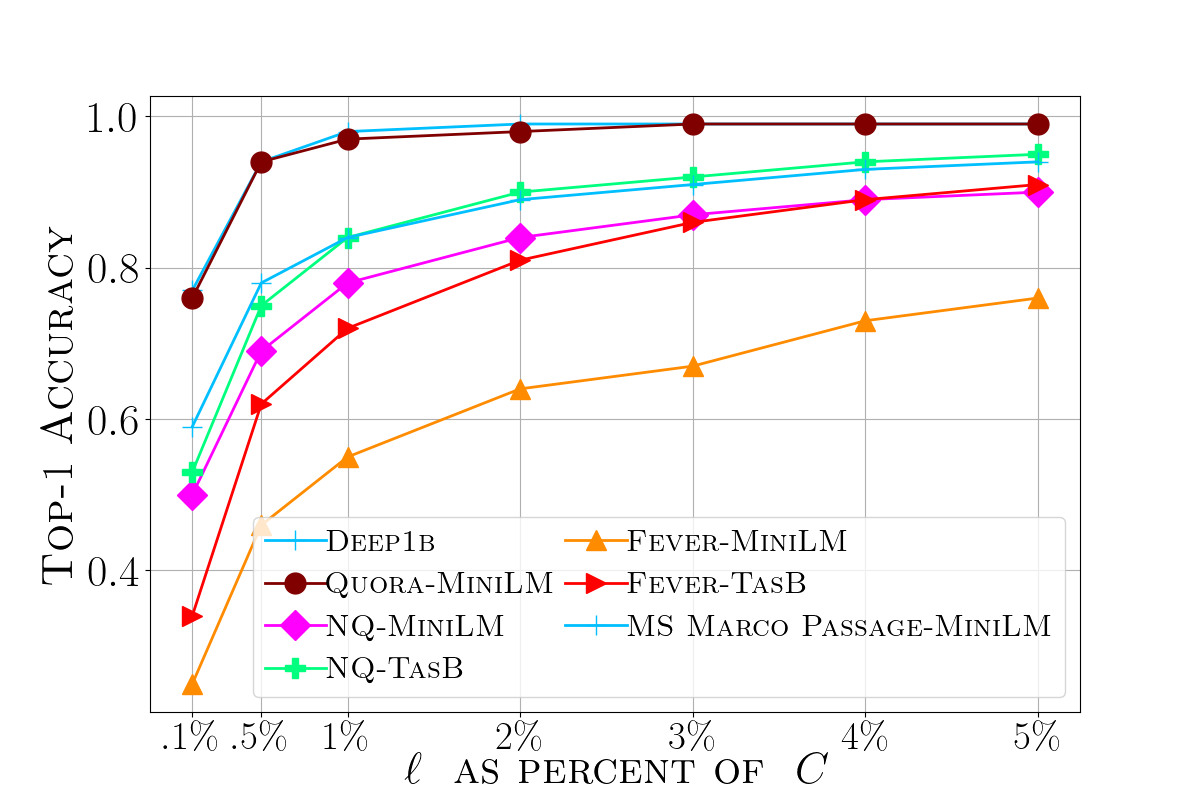
\includegraphics[width=0.5\linewidth]{figures/clustering-performance-mips.png}
    }
    \subfloat[\textsc{NN}]{
        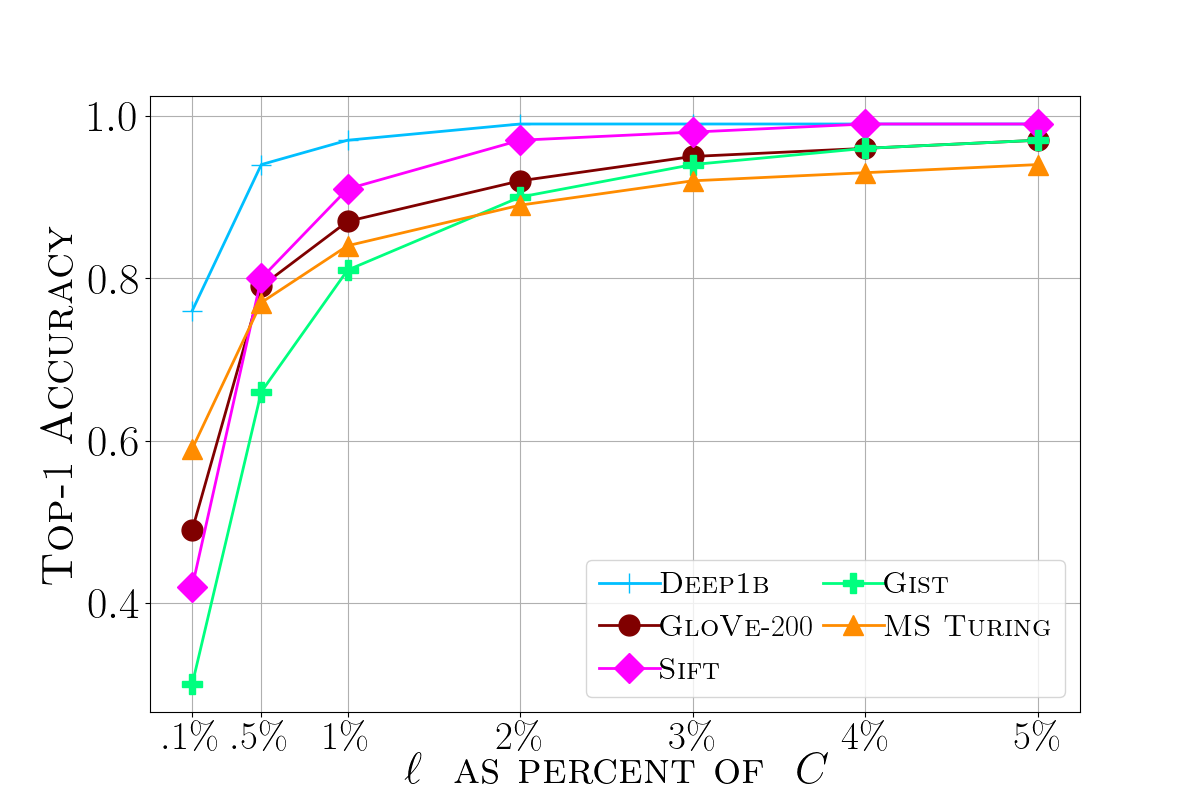
\includegraphics[width=0.5\linewidth]{figures/clustering-performance-nn.png}
    }
    \caption{Performance of the clustering-based retrieval method on various real-world collections,
    described in Appendix~\ref{appendix:collections}.
    The figure shows top-$1$ accuracy versus the
    number of clusters, $\ell$, considered by the routing function $\tau(\cdot)$ as a percentage of
    the number of clusters $C$. In these experiments, we set $C = \sqrt{m}$, where $m=\lvert \mathcal{X} \rvert$ is the size of the collection, and use spherical KMeans (MIPS) and standard KMeans (NN)
    to form clusters.}
    \label{figure:ivf:clustering-performance}
\end{figure}

However, to date, no formal analysis has been presented to quantify the retrieval error.
The choice of $\zeta$ and $\tau$, too, have been left largely unexplored, with KMeans and
Equation~(\ref{equation:ivf:centroid-based-routing}) as default answers. It is, for example, not known
if KMeans is the right choice for a given $\delta$. Or, whether clustering with
spillage, where each data point may belong to multiple clusters, might reduce the overall
error, as it did in Spill Trees. It is also an open question if,
for a particular choice of $\zeta$ and $\delta$, there exists
a more effective routing function---including learnt functions tailored to
a query distribution---that uses higher-order statistics from the cluster distributions.

In spite of these shortcomings, the algorithmic framework above contains a
fascinating insight that is actually useful for a rather different end-goal:
vector compression, or more precisely, \emph{quantization}.
We will unpack this connection in Chapter~\ref{chapter:quantization}.

\section{Closing Remarks}
This chapter departed entirely from the theme of this monograph.
Whereas we are generally able to say something intelligent about
trees, hash functions, and graphs, top-$k$ retrieval by clustering
has emerged entirely based on our intuition that data points naturally
form clusters. We cannot formally determine, for example, the behavior
of the retrieval system as a function of the clustering algorithm itself,
the number of clusters, or the routing function. All that must be determined empirically.

What we do observe often in practice, however, is that clustering-based
top-$k$ retrieval is \emph{efficient}~\citep{kmeanslsh,auvolat2015clustering,bruch2023bridging,pq},
at least in the case of Nearest Neighbor search with Euclidean distance,
where KMeans is a theoretically appropriate choice. It is efficient in the sense that
retrieval accuracy often reaches an acceptable level after probing
a few top-ranking clusters as identified by
Equation~(\ref{equation:ivf:centroid-based-routing}).

That we have a method that is efficient in practice, but
its efficiency and the conditions under which it is efficient are unexplained,
constitutes a substantial gap and thus presents multiple consequential open questions.
These questions involve optimal clustering, routing, and bounds on retrieval accuracy.

\bigskip

When the distance function is the Euclidean distance and our
objective is to learn the Voronoi regions of data points, the KMeans
clustering objective makes sense. We can even state formal results
regarding the optimality of the resulting clustering~\citep{kmeansplusplus_2007}.
That argument is no longer valid when the distance function is based on inner product,
where we must learn the inner product Voronoi cones, and where some points
may have an empty Voronoi region. What objective we must optimize for MIPS,
therefore, is an open question that, as we saw in this chapter,
has been partially explored in the past~\citep{scann}.

Even when we know what the right clustering algorithm is, there is still
the issue of ``balance'' that we must understand how to handle. It would,
for example, be far from ideal if the clusters end up having very different
sizes. Unfortunately, that happens quite naturally if the data points have
highly variable norms and the clustering algorithm is based on KMeans:
Data points with large norms become isolated, while vectors with small
norms form massive clusters.

\bigskip

What has been left entirely untouched is the routing machinery.
Equation~(\ref{equation:ivf:centroid-based-routing}) is the \emph{de facto}
routing function, but one that is possibly sub-optimal.
That is because, Equation~(\ref{equation:ivf:centroid-based-routing})
uses the mean of the data points within a cluster as the representative
or \emph{sketch} of that cluster. When clusters are highly concentrated
around their mean, such a sketch accurately reflects the potential of each
cluster. But when clusters have different shapes, higher-order statistics
from the cluster may be required to accurately route queries to clusters.

So the question we are faced with is the following: What is a good sketch
of each cluster? Is there a \emph{coreset} of data points within each cluster
that lead to better routing of queries during retrieval? Can we quantify the
probability of error---in the sense that the cluster containing the optimal
solution is not returned by the routing function---given a sketch?

We may answer these questions differently if we had some idea of what the query
distribution looks like. Assuming access to a set of training queries, it may
be possible to learn a more optimal sketch using supervised learning methods.
Concepts from learning-to-rank~\citep{bruch2023fntir}
seem particularly relevant to this setup. To see how, note that the
outcome of the routing function is to
identify the cluster that contains the optimal data point for a query.
We could view this as ranking clusters with respect to a query,
where we wish for the ``correct'' cluster to appear at the top
of the ranked list. Given this mental model, we
can evaluate the quality of a routing function using any of the many
ranking quality metrics such as Reciprocal Rank (defined as the reciprocal
of the rank of the correct cluster).
Learning a ranking function that maximizes Reciprocal Rank
can then be done indirectly by optimizing a custom
cross entropy-based surrogate, as proved by~\cite{bruch2019xendcg} and~\cite{bruch2021xendcg}.

\bigskip

Perhaps the more important open question is understanding when clustering
is efficient and why. Answering that question may require exploring the connection
between clustering-based top-$k$ retrieval, branch-and-bound algorithms, and LSH.

Take any clustering algorithm, $\zeta$. If one could show formally
that $\zeta$ behaves like an LSH family, then clustering-based top-$k$ retrieval
simply collapses to LSH. In that case, not only do the results from that literature
apply, but the techniques developed for LSH (such as multi-probe LSH) too
port over to clustering.

Similarly, one may adopt the view that finding the top cluster is a series
of decisions, each determining which side of a hyperplane a point falls.
Whereas in Random Partition Trees or Spill Trees, such decision hyperplanes were
random directions, here the hyperplanes are correlated.
Nonetheless, that insight could help us produce clusters with spillage, where
data points belong to multiple clusters, and in a manner that helps reduce
the overall error.

\bibliographystyle{abbrvnat}
\bibliography{biblio}
